
% this file is called up by thesis.tex
% content in this file will be fed into the main document

%: ----------------------- introduction file header -----------------------
%\begin{savequote}[50mm]
%Now this is not the end. It is not even the beginning of the end. But it is, perhaps, the end of the beginning. 
%\qauthor{Winston Churchill}
%\end{savequote}

%---- formato chapter

% \chapter format
\titleformat{\chapter}[display]%		
% Label and title options
{\filleft}%
% Label format and text
{\color{Gray}{\filleft\small{\bfseries CHAPTER}} {\linebreak\fontsize{90}{90}\selectfont\selectfont {\bfseries \thechapter}}}	   
% Label and title distance
{2ex}
% Title format
{\vspace{2ex}\bfseries \fontsize{30}{30}\selectfont}%
% Space between title and text
\titlespacing{\chapter}{3mm}{*10}{15mm}[3mm]

%---- fin formato chapter

\chapter{Conclusions and future work}
\label{cha:ConclusionsEN}

% the code below specifies where the figures are stored
\ifpdf
    \graphicspath{{6_conclusion/figures/PNG/}{6_conclusion/figures/PDF/}{6_conclusion/figures/}}
\else
    \graphicspath{{6_conclusion/figures/EPS/}{6_conclusion/figures/}}
\fi

%\textbf{This is the English version of Chapter~\ref{cha:Conclusions}.}
%\bigskip

This chapter presents the conclusions and the future works derived from this research.


%------------------------------------------------------------------------- 

\section{Conclusions}

This dissertation studies the use of indicators obtained from virtual learning environments activity registers to assess students’ performance in generic skills.

In order to achieve the objectives outlined  in the introductory chapter, an evaluation method called Design-Based Assessment (DBA) was proposed and two Domain-Specific Languages (DSL) were developed. The DBA method makes it possible to define a hypothesis evaluation by designing indicators based on virtual learning environments activity registers, to subsequently analyse the results of their application; if the teacher then deems it as necessary, a redefinition of the initial hypothesis may be performed, thus beginning the cycle again. On the other hand, the DSLs developed to facilitate the implementation of the method in both learning management systems based on Moodle and virtual worlds based on OpenSim are called SASQL and VWQL respectively.

The following hypotheses were formulated for the evaluation of the method and the DSLs: the DBA method allows to automatically obtain indicators from virtual learning environments (H1) and the DSLs allow teachers to design and contrast evaluation strategies from virtual learning environments activity registers (H2).

To verify these hypotheses, the DBA method along with the DSLs have been firstly implemented and used in several courses taught in the Degree in Computer Engineering at the University of Cádiz and in a case study conducted in a language course with high school students. Secondly, they were evaluated by teachers belonging to both all educational levels and all branches of knowledge.

From the results obtained from the evaluation, it is concluded that the DBA method can address the assessment of generic skills. The objective indicators of students’ interaction in virtual learning environments provided by the DBA method have been positively evaluated in the study.

In particular, there are evidences to support the following conclusions:

\begin{itemize}
\item The DBA method is suitable to design and contrast assessment strategies from the virtual learning environments activity registers. The DBA method features which are most valued in the study are its adaptability, its systematicity and its flexibility. 
\item The DSL facilitates the implementation of the DBA method. The DSL features which are most valued are its ease of learning, its effectiveness, its efficiency and its reusability. In addition, both the queries that can be defined with the DSL and the results that the system returns are easily interpretable by most of the surveyed teachers, thus demonstrating that the DSL can be used by teachers without programming skills.
\end{itemize}
% ----------------------------------------------------------------------

\subsection{Scope}

The scope of the aforementioned conclusions should be considered when situations similar to those described in this research concur. However, it cannot be confirmed that a situation is within their scope when circumstances like the following are occurring:

\begin{itemize}
\item Teachers do not include modules in their virtual courses that generate activity in the virtual learning registers or, if even with these modules, teachers do not encourage their students to use them.
\item The registers containing information on the activity generated by students in virtual learning environments cannot be accessed neither through direct connection nor through backup. In this case, a method based on Linked Open Data~\cite{ruiz2015framework} could be applied to turn the activity registered in the virtual learning environment into open data. 
\end{itemize}

\subsection{Threats to validity}

The main threat to validity is related to the sample of teachers who participated in the evaluation of the proposals. The DBA method and the DSLs have been tested and evaluated in an adequate sample size~\cite{oates2006researching}. However, the majority of subjects are teachers who, even without a digital profile, share their interest in educational innovation, new technologies and their application in improving learning processes. Forums in which both the DBA method and the DSLs  were presented were conferences, seminars and courses that the participants went willingly. Hence, it is still required to know the evaluation of teachers who a priori do not have these concerns and / or tend to stay out of these events. 

On the other hand, the fact that the DBA method, using the tools implemented, has been tested only in two specific virtual learning environments is also considered a threat to its validity. These environments are the learning management system Moodle (through SASQL) and virtual worlds based on OpenSim (by VWQL). The DSLs should be adapted to be used in the analysis of interactions produced in other virtual learning environments such as collaborative development platforms, digital content repositories and augmented reality applications.

\section{Contributions} \label{eva:contribucionesEN}

	The main contributions made during the preparation of this research are detailed below:

	\subsection*{Journal publications}


Journal article in \emph{Computers in Human Behaviour} (2014), entitled \textbf{``Scalability of assessments of wiki-based learning experiences in higher education''}~\cite{palomo2014scalability} (\emph{ISI JCR 2014: Q1, T1})

\begin{quote}Seven case studies of assessment in wikis in higher education were presented in this article. Among those experiences, two tools that supported a scalable way to address assessment of various abilities of students from work in MediaWiki wikis stand out. The different configurations and methodologies of the tools were analysed and compared in the context of each of the seven case studies provided. One of the tools used was AssessMediaWiki, which by self-, hetero- and peer-evaluation procedures supplemented the quantitative approach provided by the StatMediaWiki tool with a qualitative view.\end{quote}

\noindent
Journal article in \emph{International Journal of Engineering Education} (2015), entitled \textbf{``A Domain Specific Language for Online Learning Competence Assessments''}~\cite{Balderas:2015} (\emph{ISI JCR 2015: Q3, T3})

\begin{quote}This article presented the use of SASQL to design assessments based on indicators derived from the students’ interaction in two case studies carried out in two virtual courses. These indicators were used to assist in the assessment of students’ performance on the following generic skills: leadership, interpersonal skills and ability to be critical and self-critical.\end{quote}

\noindent
Journal article submitted to \emph{Journal of Information Technology Research} (2016) invited after presenting in Technological Ecosystem for Enhancing Multiculturality (TEEM 2015)~\cite{balderas2015domain}, entitled \textbf{``Retrieving Objective Indicators from Student Logs in Virtual Worlds''} (SCImago SJR 2015: Q4)

\begin{quote}Students’ behaviour in a virtual world based on OpenSim was analysed in this paper, using EvalSim and VWQL. Assessments were designed and indicators were obtained from students’ interaction in the virtual world. These indicators were used to establish a fairer comparison of students’ performance and draw conclusions on the analysis of the learning processes.\end{quote}

%\fcolorbox{grey}{grey}{\parbox{0.7\textwidth}{%
%   \color{black}%
% % Para cuadro gris
%}}

	\subsection*{Conference proceedings}

Oral communication presented at the \emph{IX Simposio Pluridisciplinar sobre Diseño, Evaluación y Descripción de Contenidos Educativos (SPDECE 2012)}, entitled ``\textbf{Qualitative assessment of wiki-based learning processes}''~\cite{Balderas:2012}

\begin{quote}AsssessMediaWiki was introduced and applied in this paper in order to support peer-, hetero- and self-assessment procedures. These procedures were used in students’ contributions to a wiki based on MediaWiki. Students assessed their peer contributions from the aspects of a rubric about the specific work that their peers should perform, whereas the lecturer used the differences in assessments made by the students to assess their critical capacities.\end{quote}

\noindent
Poster presented at the \emph{8th European Conference on Technology Enhanced Learning (EC-TEL 2013)}, entitled ``\textbf{A Generative Computer Language to Customize Online Learning Assessments}''~\cite{Balderas:2013}

\begin{quote}EvalCourse and SASQL syntax were presented in this contribution, along with a simple example.\end{quote}

\noindent
Oral communication presented at the \emph{4th International Workshop on Software Engineering for E-learning (ISELEAR’13)}, held within \emph{I International Conference on Technological Ecosystem for Enhancing Multiculturality (TEEM 2013)}, entitled ``\textbf{A generative computer language to customize online learning assessments}''~\cite{balderas2013generative}

\begin{quote}EvalCourse and SASQL were applied to a case study to obtain indicators on students’ activity in a virtual course. These indicators were used to support the assessment of students’ performance on the generic competences of leadership, planning and time management and teamwork.\end{quote}

\noindent
Oral communication presented at the \emph{International Symposium on Computers in Education (SIIE 2014)}, entitled ``\textbf{Domain-driven competence assessment in virtual learning environments. Application to planning and time management skills}''~\cite{balderas2014domain}

\begin{quote}This work compares two approaches to deal with the assessment of generic skills. The first approach is based on a model-driven architecture where EvalCourse and SASQL are applied, while the second approach is based on a Web ReST service called Gescompeval\_MD, which allows lecturers to flag the skills that will be developed in each activity. The results of jointly applying both approaches show that they are complementary, since while the web service provides a much more detailed feedback, the model-driven approach is much more scalable when the number of students increases and generic skills have to be assessed.\end{quote}

\noindent
Oral communication presented at the \emph{6th International Workshop on Software Engineering for E-learning (ISELEAR’15)}, held within \emph{III International Conference on Technological Ecosystem for Enhancing Multiculturality (TEEM 2015)}, entitled ``\textbf{A Domain Specific Language to retrieve objective indicators for foreign language learning in virtual worlds}''~\cite{balderas2015domain}

\begin{quote}Both VWQL and a pilot experience of its application in a language course were presented in this paper. Several assessments based on indicators were designed from students’ interactions in a virtual world. These indicators were applied to the assessment of the ‘communication in a second language’ generic skill.\end{quote}

	\subsection*{Other contributions}

	This section presents not previously described contributions from the work developed in this thesis. These contributions are divided into two main categories. The first one, called \emph{methodological contributions}, includes the proposed method. The second category, called \emph{software contributions}, encompasses the tools that have been developed to implement the method.

	\paragraph*{Methodological contributions}

	\begin{itemize}
	\item DBA method: assessment method based on the design of indicators obtained from the information stored in the virtual learning environments activity registers.
	\end{itemize}

	\paragraph*{Software contributions}

	\begin{itemize}
	\item AssessMediaWiki system~\cite{Balderas:2012}: web tool that supports the assessment of contributions made in a wiki based on MediaWiki, through peer-, self- and hetero-assessment procedures.
	\item EvalCourse system and SASQL query language~\cite{Balderas:2013,balderas2013generative,Balderas:2015}: DSL oriented to applying the DBA method in Moodle-based learning management systems.
	\item EvalSim system and VWQL query language~\cite{balderas2015domain}: DSL oriented to applying the DBA method in OpenSim-based virtual worlds.

	\end{itemize}

\section{Future work}

Although while performing this work, the challenges initially raised have been overcome, some problems and new challenges have been detected. Despite them not having been addressed, it is fair to say that in many cases they would help in complementing this thesis.

These future works are listed below:
\begin{itemize}
\item Adaptation and extension of the DSLs that have been presented in this thesis so that they can be used in obtaining indicators of other virtual learning environments such as collaborative development platforms, digital content repositories, and augmented reality applications.
\item The addition of indicators based on the application of \emph{social network analysis} (SNA) techniques to virtual learning environments. Students worked in pairs in the wiki of a Moodle-based learning management system, with each pair performing their work in a wiki page. Once the activity was finished, the graph shown in Figure 1 was obtained using SNA techniques. In this graph, the central node represents the teacher. It can be seen how initially the teacher created the main section, while students placed links to their pages in this main page (edge ​​joining the peripheral nodes to the central node). The remaining edges joining two peripheral nodes typically represent students who worked together on a page. The size of the nodes represents the amount of work done by each student. The indicators obtained through this analysis could be applied in the assessment of generic skills related to teamwork and interaction between team members.
\end{itemize}

\begin{figure}[h]
  \begin{center}
    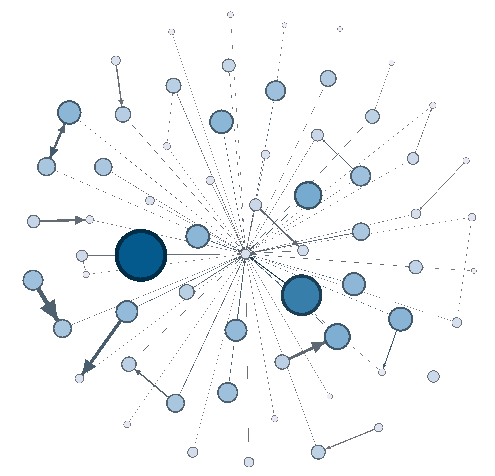
\includegraphics[scale=0.5]{SNA-Grafo-Wiki-SD.png}
  \end{center}
  \caption{Resulting graphic of applying techniques to SNA Moodle wiki}
  \label{fig:SNAWikiEN}
\end{figure}

\begin{itemize}
\item The integration of the DSLs into virtual learning environments. Instead of being integrated into virtual learning environments, the DSLs presented in this paper are connected to them in order to obtain the indicators. Sometimes the settings of this connection can represent a complex task for teachers with little computer programming skills. Thus, it would be interesting to integrate DSL environments within the supervisor profile in the virtual learning environment. To do this, the latest version of Xtext could be used in the server, as it incorporates XtextServlet to respond to customer requests. This way the language parser for use via HTTP could be implemented. On the client side you could use a JavaScript  web editor (CodeMirror~\footnote{\url{http://codemirror.net}}, Orion~\footnote{\url{https://orionhub.org}}, etc.).
\item The creation of a visual version of the DSL. Despite having tried to develop a simple language with a syntax close to the domain of teaching, there may be teachers who still feel uncomfortable when coding queries. In this case, a visual version of the DSL could be more attractive, especially to teachers with this profile. The development of the visual DSL could be performed with the Sirius Eclipse tool~\footnote{\url{https://eclipse.org/sirius}}.
\item Creating a repository that maps activities to be performed by students in virtual learning environments, indicators that these activities generate and generic skills that can be assessed with these indicators. The lecturers who have applied the method have proposed different indicators for the assessment of skills. Should they share their skill assessment hypothesis based on indicators, the community of lecturers could take advantage of them to see how other teachers do and assess their students in these skills either by using those assumptions as they are or by redefining them.
\end{itemize}


% ----------------------------------------------------------------------
